\section{Code Validation}
A set of simulations was performed to evaluate the accuracy and reliability of Omnisoot in predicting soot formation. The aerosol dynamics models were validated by comparing the results of the population balance models implemented in Omnisoot with discrete element method (DEM) simulations reported in the literature. In addition, carbon and hydrogen mass and energy balances were rigorously assessed to ensure that residuals remain within the bounds of acceptable numerical error.

\subsection{Coagulation}
The collision kernels and their corresponding interpolation schemes implemented in Omnisoot were validated by comparing the computed collision frequencies across a wide range of Knudsen numbers with reference DEM results~\citep{goudeli2015coagulation} shown in Figure~\ref{fig:kernelvalid}.
Additionally, two test cases were set up to validate the coagulation sub-model of MPBM and SPBM in the free-molecular\footnote{\href{https://github.com/mohammadadib-cu/omnisoot-cv/tree/main/validations/coagulation/free_molecular}{https://github.com/mohammadadib-cu/omnisoot-cv/tree/main/validations/coagulation/free\_molecular}} and continuum \footnote{\href{https://github.com/mohammadadib-cu/omnisoot-cv/tree/main/validations/coagulation/continuum}{https://github.com/mohammadadib-cu/omnisoot-cv/tree/main/validations/coagulation/continuum}} regimes. An adiabatic CVR with a volume of 1~$\mathrm{m}^3$ was initialized with $2.6261 \times 10^{18}$ spherical particles with the initial diameter of 2~nm and 668~nm for the free-molecular and continuum cases, respectively. The initial temperature in the free-molecular and continuum simulations are 1800~K and 300~K, respectively.
 
The particles collide and grow in size through coagulation in both simulations, without inception, surface growth, or oxidation. Figure~\ref{fig:coagvalid_Nd} demonstrates the evolution of ${N_{agg}}$, ${N_{pri}}$, ${d_m}$, and ${d_g}$ as predicted by MPBM and SPBM in the free-molecular regime, which are in good agreement with DEM results~\citep{kholghy2021surface}. ${N_{pri}}$ is conserved during coagulation, resulting in identical flat trends for both models. In contrast, ${N_{agg}}$ decreases over time, with a faster decay observed in SPBM due to its treatment of agglomerate polydispersity, which leads to a higher collision frequency compared to MPBM. Therefore, $d_m$ and $d_g$  predicted by SPBM, shown in Figure~\ref{fig:coagvalid_Nd}b, are slightly larger than those predicted by MPBM.


The MPBM model cannot resolve the particle size distribution (PSD) due to the monodispersity assumption. In contrast, the SPBM tracks the number concentration of particles in discrete sections, allowing the construction of an evolving PSD, calculation of mean properties, and assessment of the size distribution spread during coagulation. Figure~\ref{fig:coagvalid_psd} shows the evolution of the non-dimensional particle size distribution (PSD) from $t=$1 ms to 500 ms for the free-molecular and continuum simulations. The PSD is plotted as a function of the normalized concentration, ${\Psi= \bar{v}n_{agg}(v,t)/N_{agg,\infty}}$ and dimensionless volume, ${\eta= v/ \bar{v}}$, where ${n_{agg}(v,t)}$ is the size distribution function of agglomerate, ${v}$ is particle volume, ${\bar{v}}$ is mean particle volume, ${N_{agg,\infty}}$ is the total number concentration of agglomerates. After the initial transient ($t>22$~ms), the PSD rapidly evolves into a full bell curve and remains unchanged, indicating the attainment of a self-preserving size distribution (SPSD). This behavior is in good agreement with DEM results and confirms the capability of the SPBM implemented in Omnisoot to capture SPSD for soot agglomerates in the free-molecular and continuum regimes, a characteristic outcome of Brownian-driven particle coagulation.


Figure~\ref{fig:coagvalid_psd}a shows the standard deviation of the mobility diameter, ${\sigma_g}$, predicted by SPBM in the free-molecular regime, which is in close agreement with DEM results. Initially, ${\sigma_g}=1$, indicating a monodisperse population, and it gradually increases, reaching a final value of 2.03, which corresponds to the characteristic standard deviation for the free-molecular regime~\citep{vemury1995self}.


\begin{figure}[H]
	\centering
	\begin{subfigure}[t]{0.4\textwidth}
		\begin{tikzpicture}
			\draw (0, 0) node[inner sep=0] 	{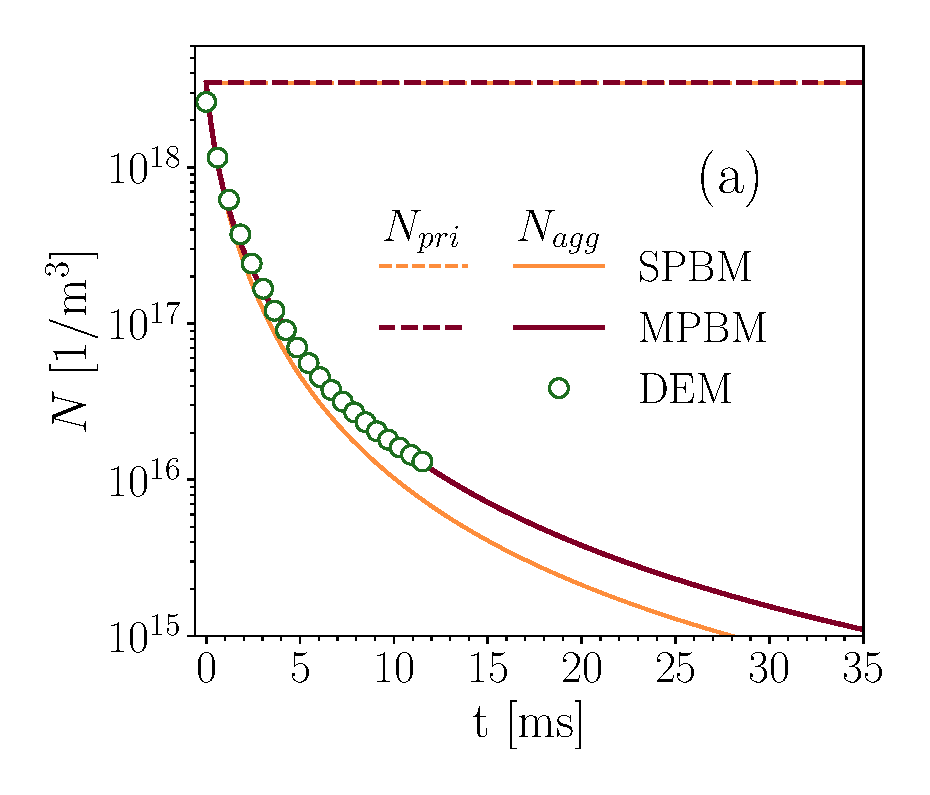
\includegraphics[width=1\textwidth]{Figures/Results/Validation/Coagulation/N_agg_pri.pdf}};
			\draw (2.1, 0.03) node {\scriptsize{\cite{kholghy2021surface}}};
		\end{tikzpicture}
	\end{subfigure}
	\begin{subfigure}[t]{0.4\textwidth}
		\begin{tikzpicture}
			\draw (0, 0) node[inner sep=0] 	{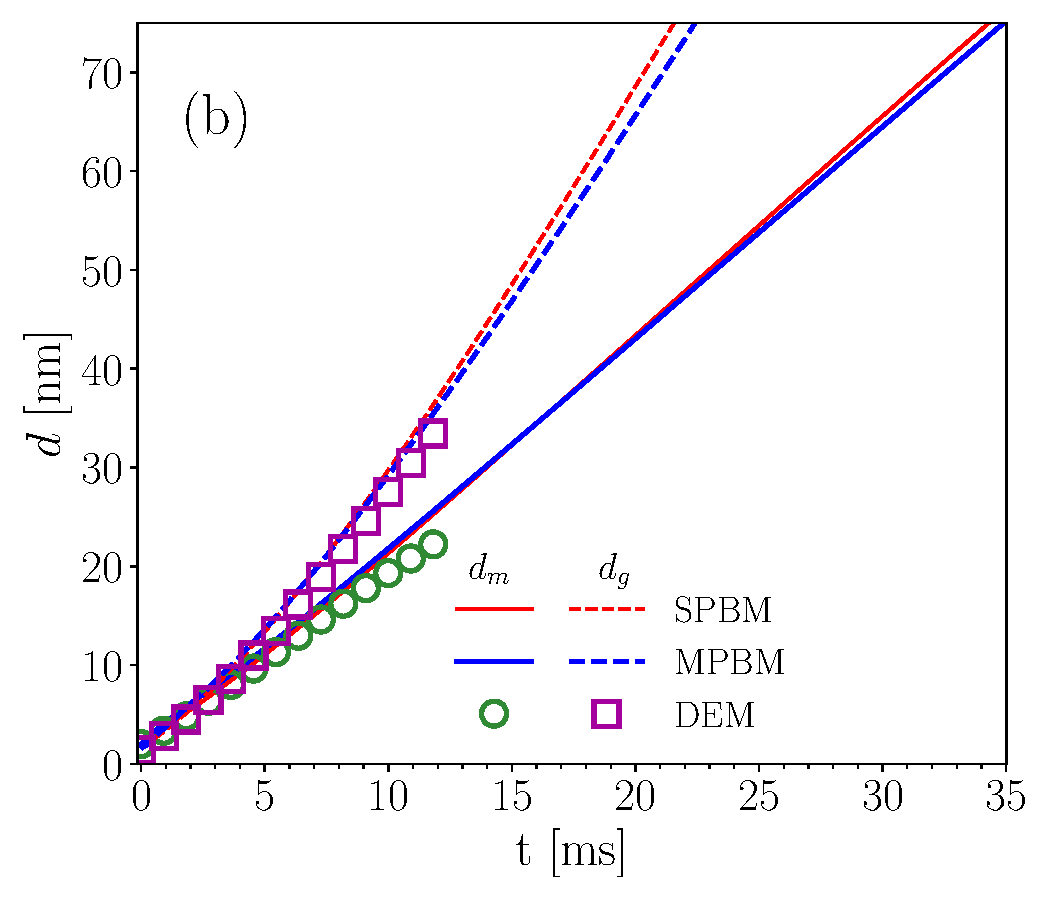
\includegraphics[width=1\textwidth]{Figures/Results/Validation/Coagulation/d_mg.pdf}};
			\draw (2.2, -1.22) node {\scriptsize{\cite{kholghy2021surface}}};
		\end{tikzpicture}
	\end{subfigure}

	\caption{The number concentration of agglomerates and primary particles (a), and mobility and gyration diameters (b) obtained by Omnisoot using MPBM and SPBM in the free-molecular regime, which are in close agreement with the DEM results~\citep{kholghy2021surface} indicating the validation of the coagulation sub-models.}
	\label{fig:coagvalid_Nd} 
\end{figure}


\begin{figure}[H]
	\centering
	\begin{subfigure}[t]{0.4\textwidth}
		\begin{tikzpicture}
			\draw (0, 0) node[inner sep=0] 	{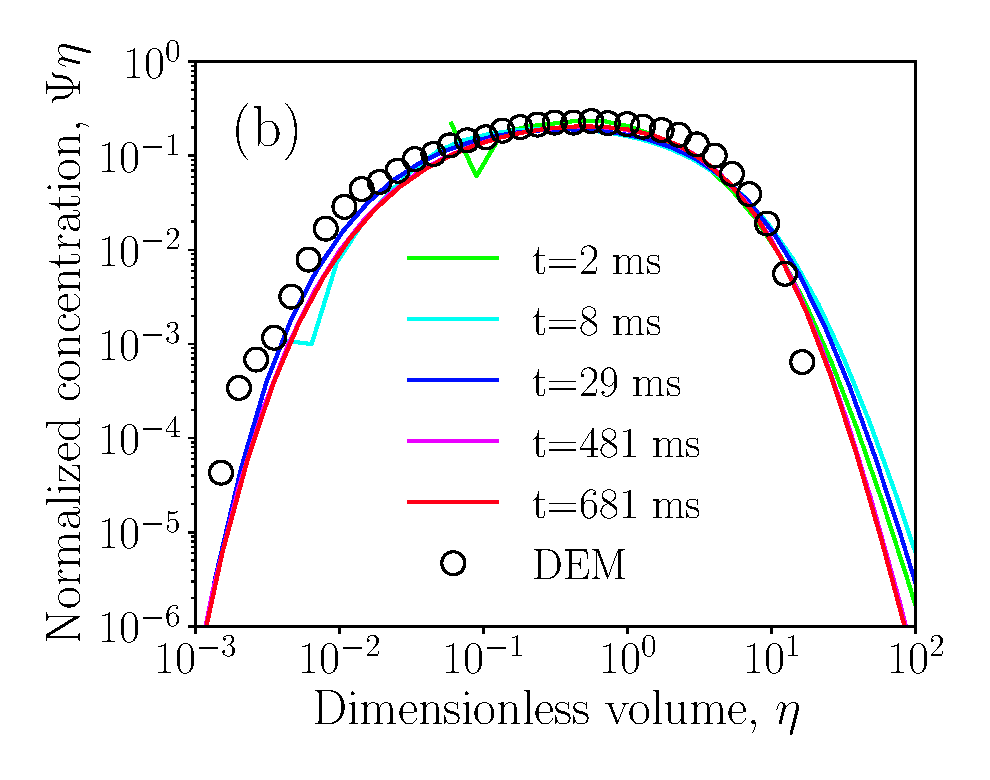
\includegraphics[width=1\textwidth]{Figures/Results/Validation/Coagulation/PSD.pdf}};
			\draw (1.3, -1.2) node {\scriptsize{\cite{goudeli2015coagulation}}};
		\end{tikzpicture}
	\end{subfigure}
	\begin{subfigure}[t]{0.4\textwidth}
		\begin{tikzpicture}
			\draw (0, 0) node[inner sep=0] 	{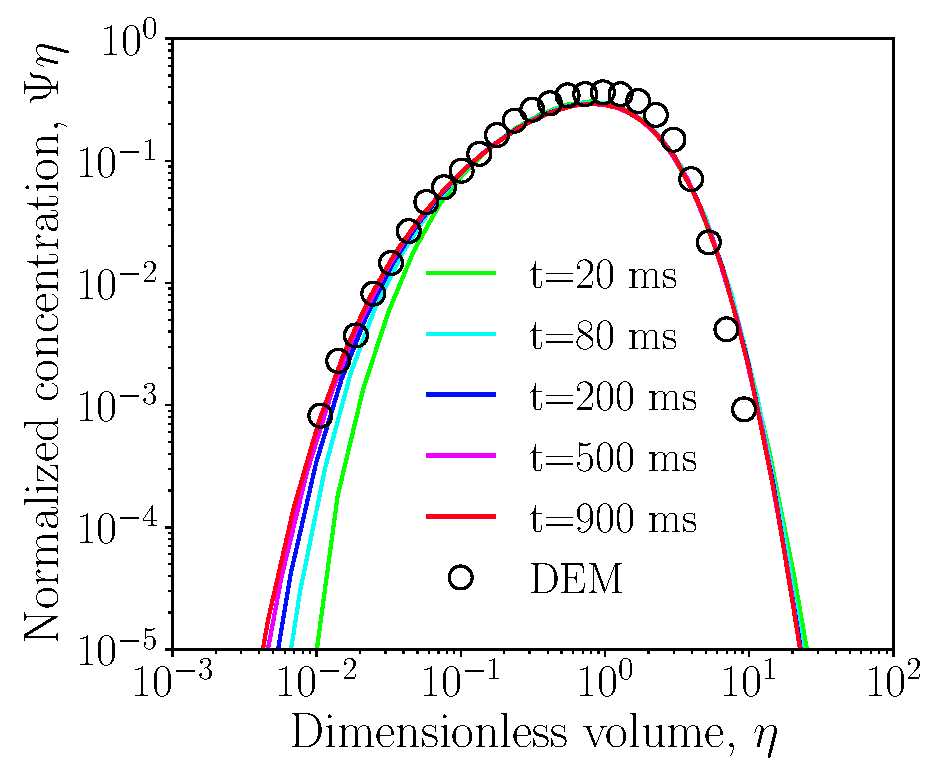
\includegraphics[width=1\textwidth]{Figures/Results/Validation/Coagulation/PSD_cont.pdf}};
			\draw (1.3, -1.22) node {\scriptsize{\cite{kholghy2021surface}}};
		\end{tikzpicture}
	\end{subfigure}
	\caption{The non-dimensional particle size distribution at different residence times in the free-molecular (a) and continuum regimes (b) overlaps after the initial transient phase, indicating the attainment of a self-preserving size distribution, which is also in good agreement with DEM results~\citep{goudeli2015coagulation}.}
	\label{fig:coagvalid_psd} 
\end{figure}

%A similar test\footnote{\href{https://github.com/mohammadadib-cu/omnisoot-cv/tree/main/validations/coagulation/continuum}{https://github.com/mohammadadib-cu/omnisoot-cv/tree/main/validations/coagulation/continuum}} was performed in the continuum regime, and the results from the SPBM were compared with those obtained from DEM. The simulation conditions were the same as in the previous case, except for the temperature, $\mathrm{T} = 600$ K, and the initial particle diameter, $d^1_p = 259$ nm. Figure~\ref{fig:coagvalid_contpsd} shows that the non-dimensional size distribution predicted by SPBM reaches the self-preserving state in good agreement with DEM results~\citep{goudeli2015coagulation}, which supports the validity of the coagulation sub-model in Omnisoot under continuum conditions.

\begin{figure}[H]
	\centering
	\begin{subfigure}[t]{0.4\textwidth}
		\begin{tikzpicture}
				\draw (0, 0) node[inner sep=0] 	{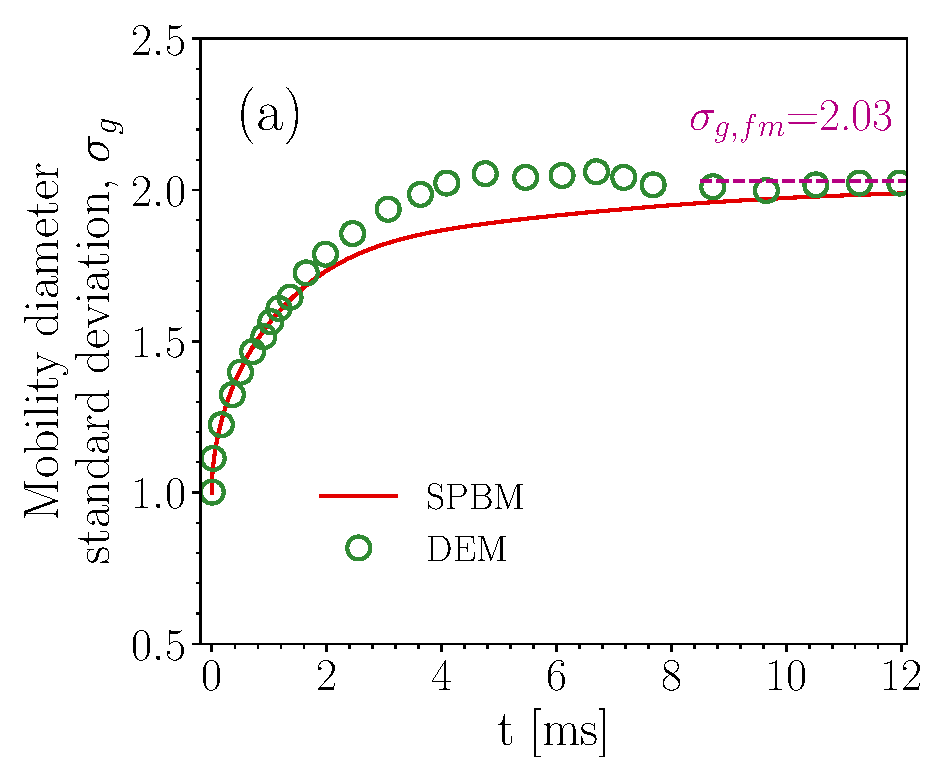
\includegraphics[width=1\textwidth]{Figures/Results/Validation/Coagulation/sigmag.pdf}};
				\draw (0.54, -1.02) node {\scriptsize{\cite{kholghy2021surface}}};
			\end{tikzpicture}
	\end{subfigure}
	\caption{Standard deviation of the mobility diameter, $\mathrm{\sigma_g}$, in the free-molecular regime obtained by SPBM is in close agreement with DEM results~\citep{kholghy2021surface}.}
	\label{fig:coagvalid_sigma} 
\end{figure}


\subsection{Elemental and Energy Balance}

\noindent To ensure the accuracy and reliability of the simulations, the conservation of elemental mass and energy was assessed across all reactor models implemented in Omnisoot. Elemental balances of carbon and hydrogen, as well as the total energy (internal or enthalpy depending on the reactor type) of the gas-particle system, were evaluated during soot formation processes under various pyrolysis and combustion conditions.
Simulations were performed using different combinations of PAH growth and particle dynamics models, and the relative errors in elemental and energy balances were monitored over time or reactor length. The residuals for all reactor configurations remained within acceptable limits (typically below $10^{-10}$), confirming that Omnisoot accurately preserves mass and energy during the coupled evolution of gas-phase and particulate species. The relative error of total carbon, hydrogen and energy in CVR, CPR, PSR, and PFR using different combinations of particle dynamics and inception models are shown in Figures~\ref{fig:constuvvalid}-\ref{fig:pfrvalid}.
 
 %Figure~\ref{fig:constuvvalid} demonstrates the relative error of total carbon, hydrogen and energy in a CVR simulation for the pyrolysis of 30\% $\mathrm{CH_4}$-$\mathrm{N_2}$ with the initial temperature and pressure of 2455 K and 3.47 atm. The relative errors are less than $10^{-11}$ for different combinations of PAH growth and particle dynamics models. The same evaluation was performed for CPR, PSR and PFR reactor and the corresponding residuals are shown in Figures~\ref{fig:cprvalid}-\ref{fig:pfrvalid}.

%\subsubsection{Constant Volume Reactor}
%The pyrolysis of 30\% $\mathrm{CH_4}$ diluted in $\mathrm{N_2}$ with the initial temperature and pressure of 2455 K and 3.47 atm, respectively, was simulated using CVR model for the residence time of 40 ms. The combination of available PAH growth and particle dynamics models leads to eight different cases that were simulated to ensure the conservation of mass and energy. Here, we focus on the total elemental balance of carbon and hydrogen because they are involved in soot processes. %The validity of models are evaluated based on relative error based on the initial mass and energy of gas. 
%Figure~\ref{fig:constuvvalid} demonstrates the relative error of total carbon, hydrogen and energy of system for different PAH growth and particle dynamics models in the constant pressure reactor that is less than $\mathrm{10^{-10}}$ for all parameters confirming the validity of model in satisfying the mass and energy balance.

%\begin{figure}[H]
%	\centering
%	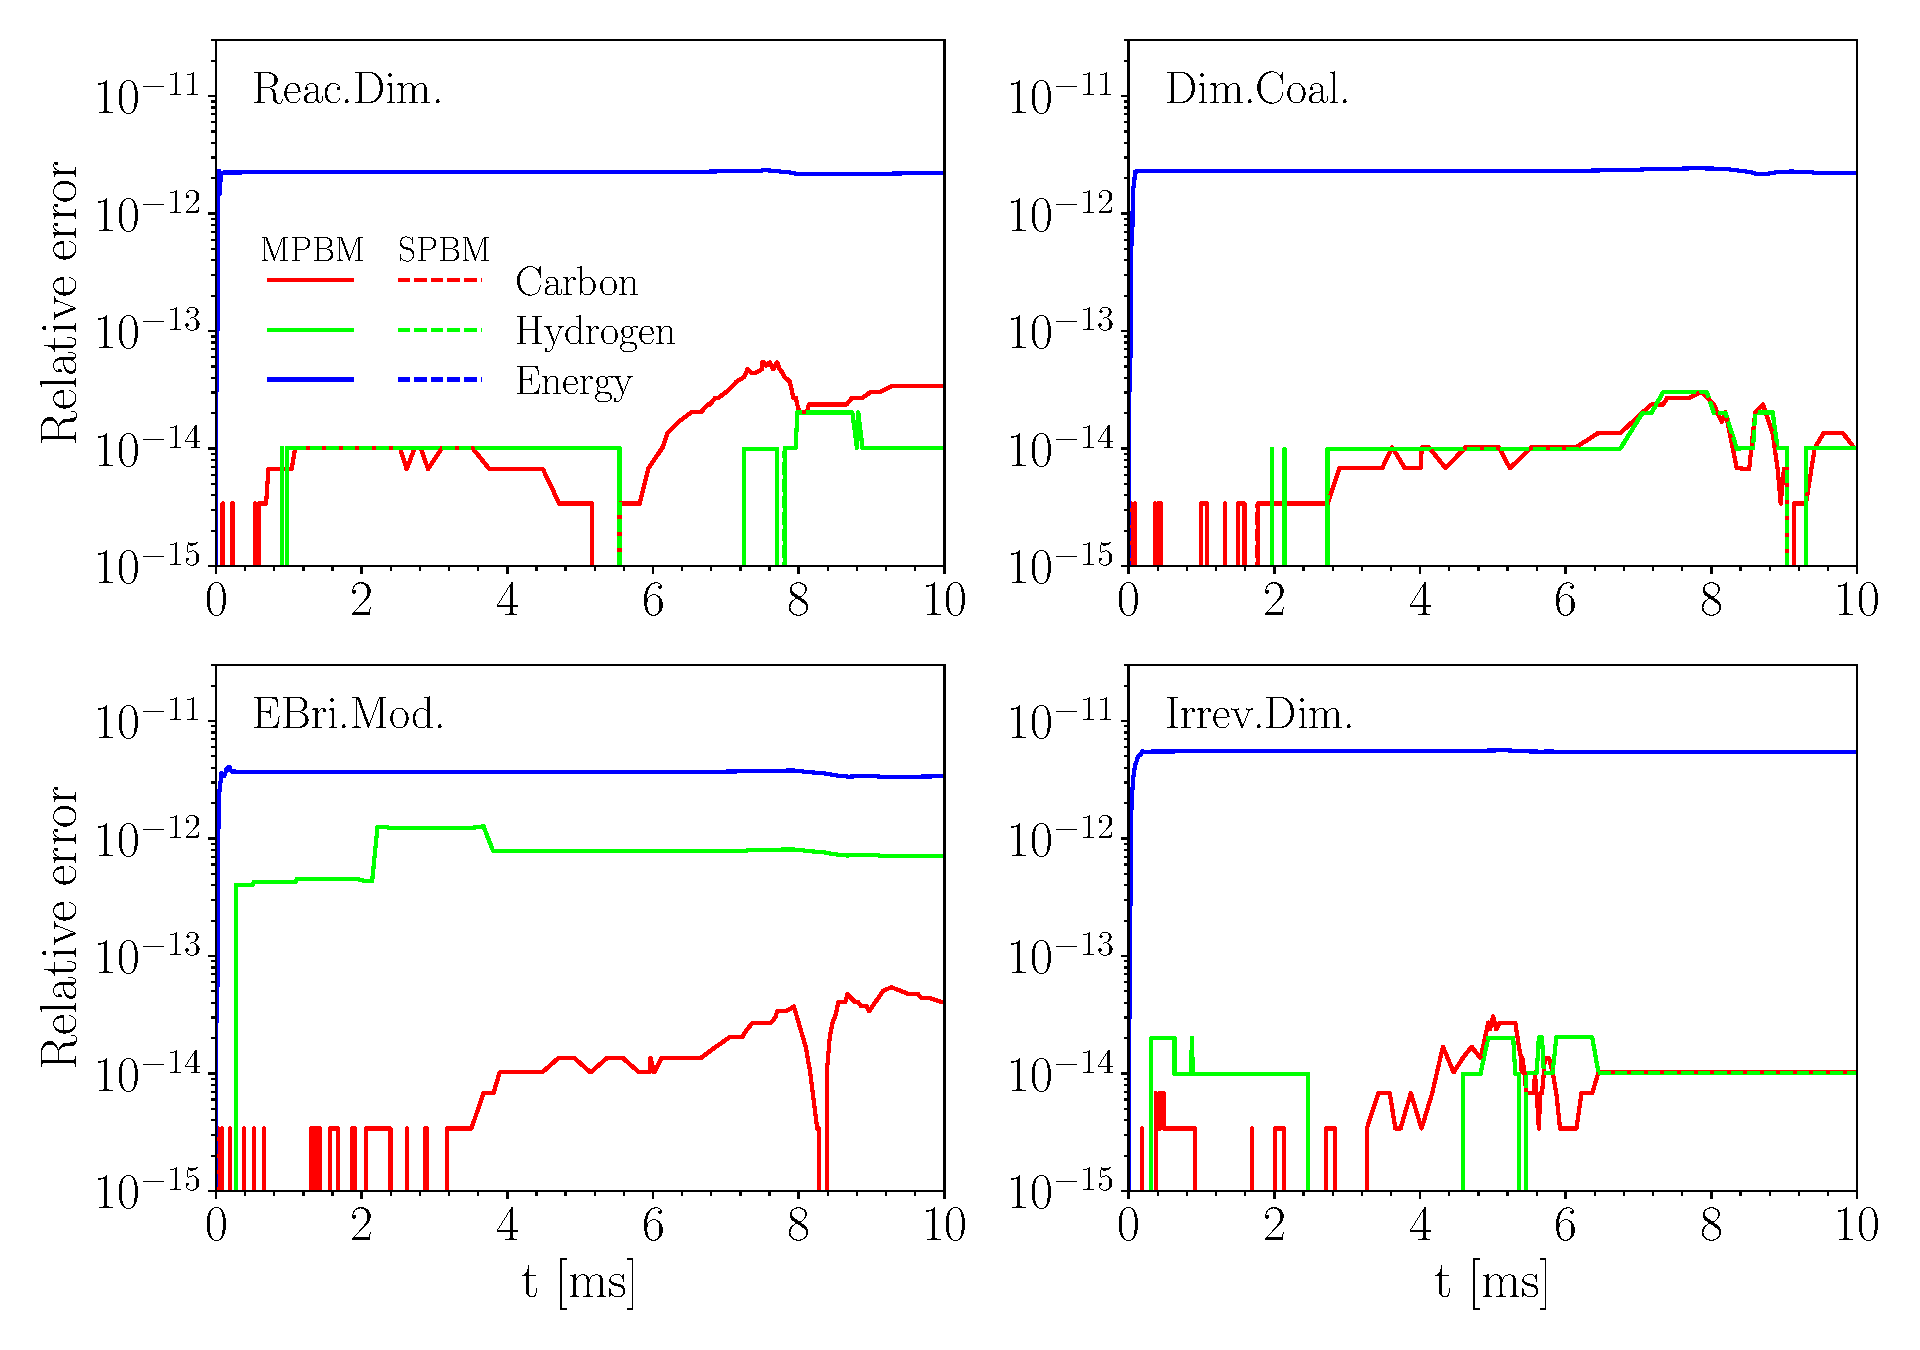
\includegraphics[width=0.8\textwidth]{Figures/Results/Validation/ConstUV/relerr_constuv.pdf}
%	\caption{The relative error (residual) of total carbon (red line) and hydrogen (green line) mass, and total internal energy residual of gas and soot (blue line) plotted against residence time during pyrolysis of 30\% $\mathrm{CH_4}$-$\mathrm{N_2}$ at 2455 K and 3.47 atm in CVR simulated using different PAH growth models along with MPBM (solid line) and SPBM (dashed line).}
%	\label{fig:constuvvalid}
%\end{figure}



